\section{Kryptologie}
\subsection{Verschlüsselung im Alltag}

Verschlüsselung ist ein Grundpfeiler der modernen Kommunikation und absolut nötig,
damit kein Unbekannter und Unbefugter private Nachrichten oder Passwörter mitlesen
kann. Ohne starke Verschlüsselungsverfahren, wäre die weitergabe sensibler Daten über
das Internet nicht möglich.

\subsection{Historische Verschlüsselungsverfahren}

\subsubsection{Caesar Chiffre}

Schon die alten Römer und viele nach ihnen erkannten, dass es durchaus von Vorteil
ist, wenn die Feinde nichts über den geheimen Schlachtplan oder die nächste Intrige
erfahren können.
Das sogenannte Caesar-Chiffre ist die einfachste Form eines symetrischen,
monoalphatischen Verschlüsselungsverfahren für Texte.
Man bestimmt eine Verschiebung zwischen 1 und 25 und ersetzt dann
alle Buchstaben des Klartexts, um den Geheimtext zu erhalten.
Kennt man die Verschiebung, so lässt sich die Nachricht auch wieder entschlüsseln.
Dieses Verfahren ist allerdings nicht sicher, weswegen es heutzutage niemand verwendet.
Um einen Buchstaben zu verschlüsseln sucht man diesen im oberen Alphabet und
ersetzt diesen dann durch den Buchstaben darunter aus dem unteren Alphabet.
Beim Entschlüsseln ist dies umgekehrt. Man ersetzt den Buchstaben im Geheimtext
durch den Buchstaben aus dem oberen Alphabet, der über der Position des Buchstabens
im unteren Alphabet ist.

\begin{lstlisting}
A B C D E F G H I J K L M N O P Q R S T U V W X Y Z
Y Z A B C D E F G H I J K L M N O P Q R S T U V W X

Klartext:     INFORMATIK
Geheimtext: GLDMPKYRGI
\end{lstlisting}

\clearpage

\subsection{Symetrische Verschlüsselung}

Symetrische Verschlüsselungsverfahren zeichnen sich dadurch aus, dass zum
Ent- und Verschlüsseln der gleiche Algorithmus und der gleiche Schlüssel verwendet
wird. Beispiele sind die Caesar Chiffre, die Vigenere Chriffe oder das Blockchiffre AES-256.

\subsubsection{Blockchriffen}

Blockchiffre Verfahren sind symetrische Verschlüsselungsverfahren,
die auch zur Verschlüsselung größerer Datenmengen genutzt werden können.
Eine besondert dieser ist, dass die zu verschlüsselnden Daten Blockweise
verschlüsselt werden und in die Verschlüsselung eines Block ein Ergebnis
der Verschlüsselung des vorigen Blocks mit eingeht.
Blockchiffren wie Advanced Encryption Standard (AES) mit hohen Bitlängen (e.g. AES-256)
sind mit heutigen Mitteln unknackbare Verfahren, weswegen dies breite Anwendung
z. B. bei Datenübertragung oder Festplattenverschlüsselung finden.

\subsubsection{Diffie-Hellman Verfahren}

Dieses von Whitfield Diffie und Martin Hellman entwickelte Verfahren ermöglicht es,
dass zwei Kommunikationspartner einen gemeinsamen, geheimen Schlüssel in Form einer Zahl
vereinbaren, auch wenn ihre Kommunikationsleitung öffentlich (unverschlüsselt ist).
Dadurch lassen sich einfach Schlüssel austauschen, um danach z. B. die Kommunikation
mit AES zu verschlüsseln.

\begin{lstlisting}
a: 0 < natürliche Zahl < p
b: 0 < natürliche Zahl < p
p: öffentliche Primzahl
g: 0 < öffentliche natürliche Zahl < p
A: öffentliche Schlüssel Alice
B: öffentliche Schlüssel Bob
K: geheimer Schlüssel, nur Bob und Alice bekannt
\end{lstlisting}

\begin{figure}[H]
    \centering
    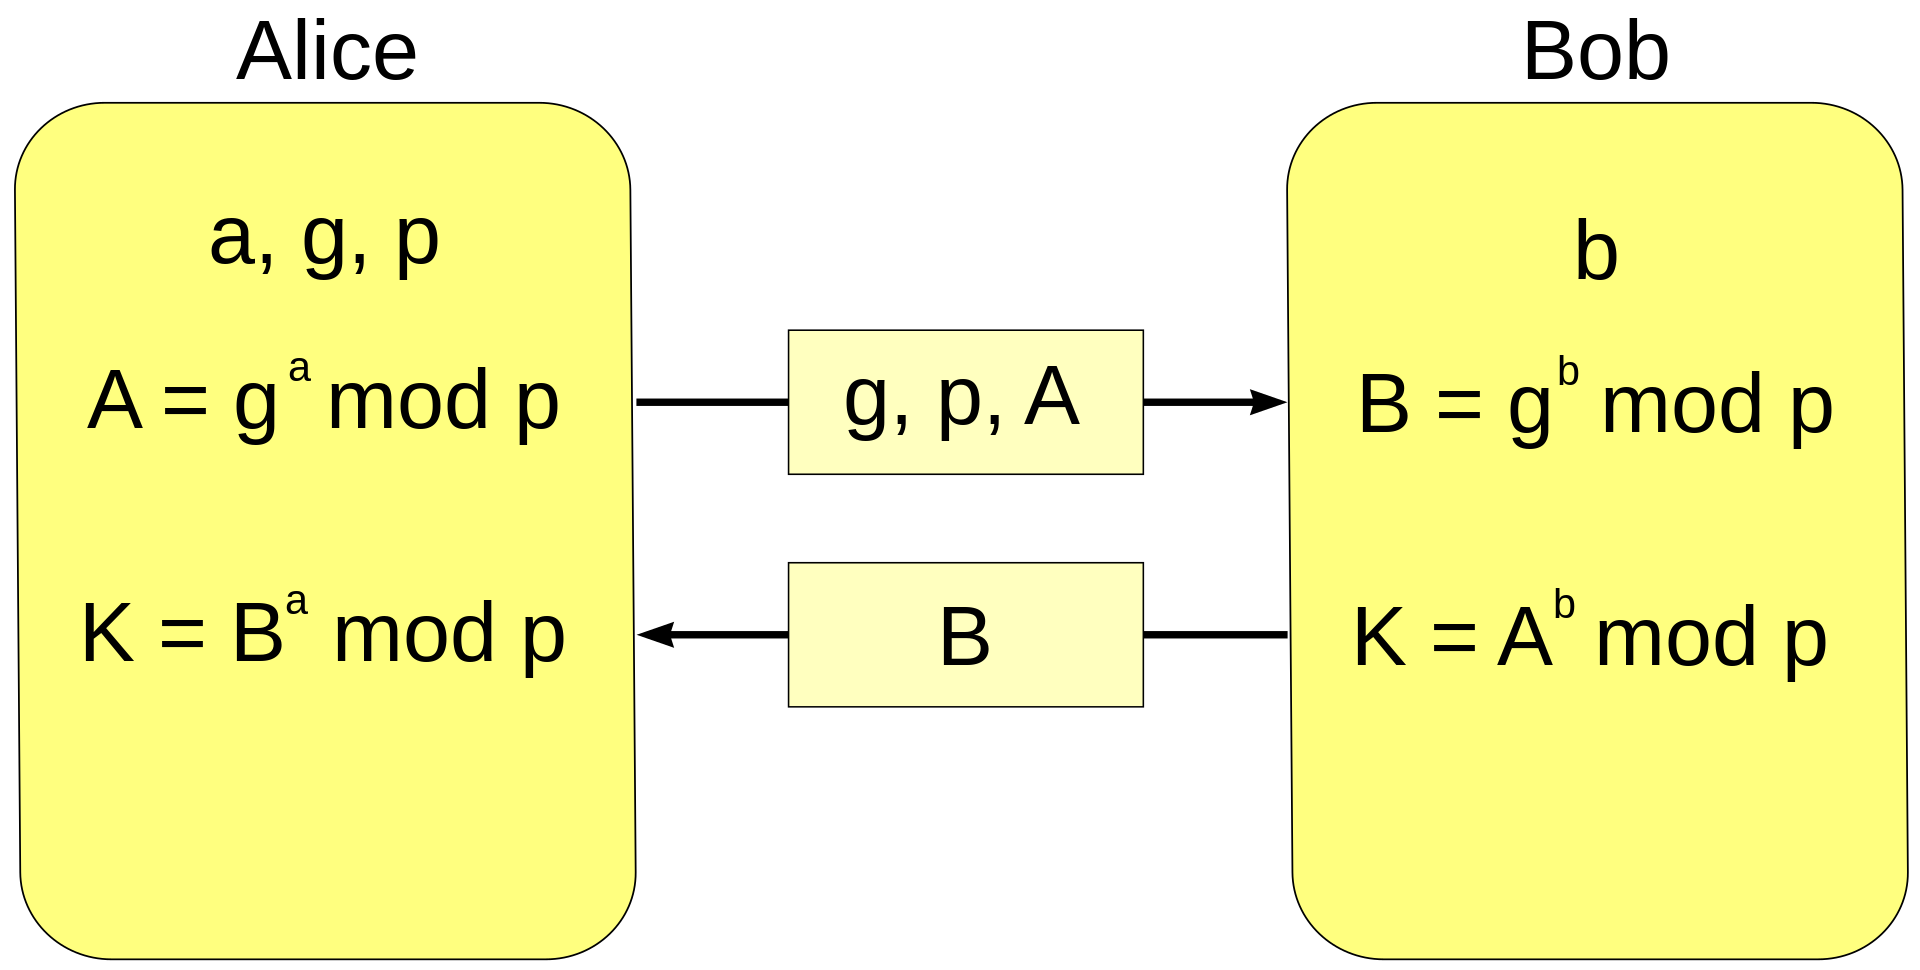
\includegraphics[width=0.6\textwidth]{images/diffie-hellman.png}
    \caption{Diffie-Hellman Schlüsseltausch}
\end{figure}

\clearpage

\subsection{Asymetrische Verschlüsselung (Public Key Cryptography)}

Die asymetrische Verschlüsselung zeichnet sich im Unterschied zur symetrischen
Verschlüsselung dadurch aus, dass es 2 Schlüssel gibt. Den einen zum Ver-, den anderen
zum Entschlüsseln. Diese beiden Schlüssel nennt man ein Schlüsselpaar.

\subsubsection{Schlüsselpaare}
Es gibt verschiedene Algorithmen, um kryptographische Schlüsselpaare zu erstellen.
Die bekanntesten und besten sind RSA und EdDSA und Variationen dieser.
Je nach Verfahren kann die Bitlänge der Schlüssel variieren, wobei höhere Bitlängen
sicherer sind. Die eigenschaften des Schlüsselpaars sind wie folgt.

\begin{lstlisting}
privater Schlüssel (öffentlicher Schlüssel (Nachricht)) = Nachricht
öffentlicher Schlüssel (privater Schlüssel (Nachricht)) = Nachricht 
\end{lstlisting}

\subsubsection{Verschlüsselung mit Public und Private Key}

Beide Kommunikationspartner erstellen ein asymetrisches Schlüsselpaar.
Anschließend übertragen beide den öffentlichen Schlüssel an den Kommunikationspartner.
Nun können Nachrichten mit dem öffentlichen Schlüssel des Partners verschüsselt werden
und nur dieser kann diese mit dem privaten Schlüssel entschlüsseln. Niemand sonst kann
so die Kommunikation mitverfolgen. Es ist auch möglich, nun einen symetrischen Schlüssel
auszutauschen und z. B. AES-256 in der weiteren Kommunikation zu verwenden.

\begin{figure}[H]
    \centering
    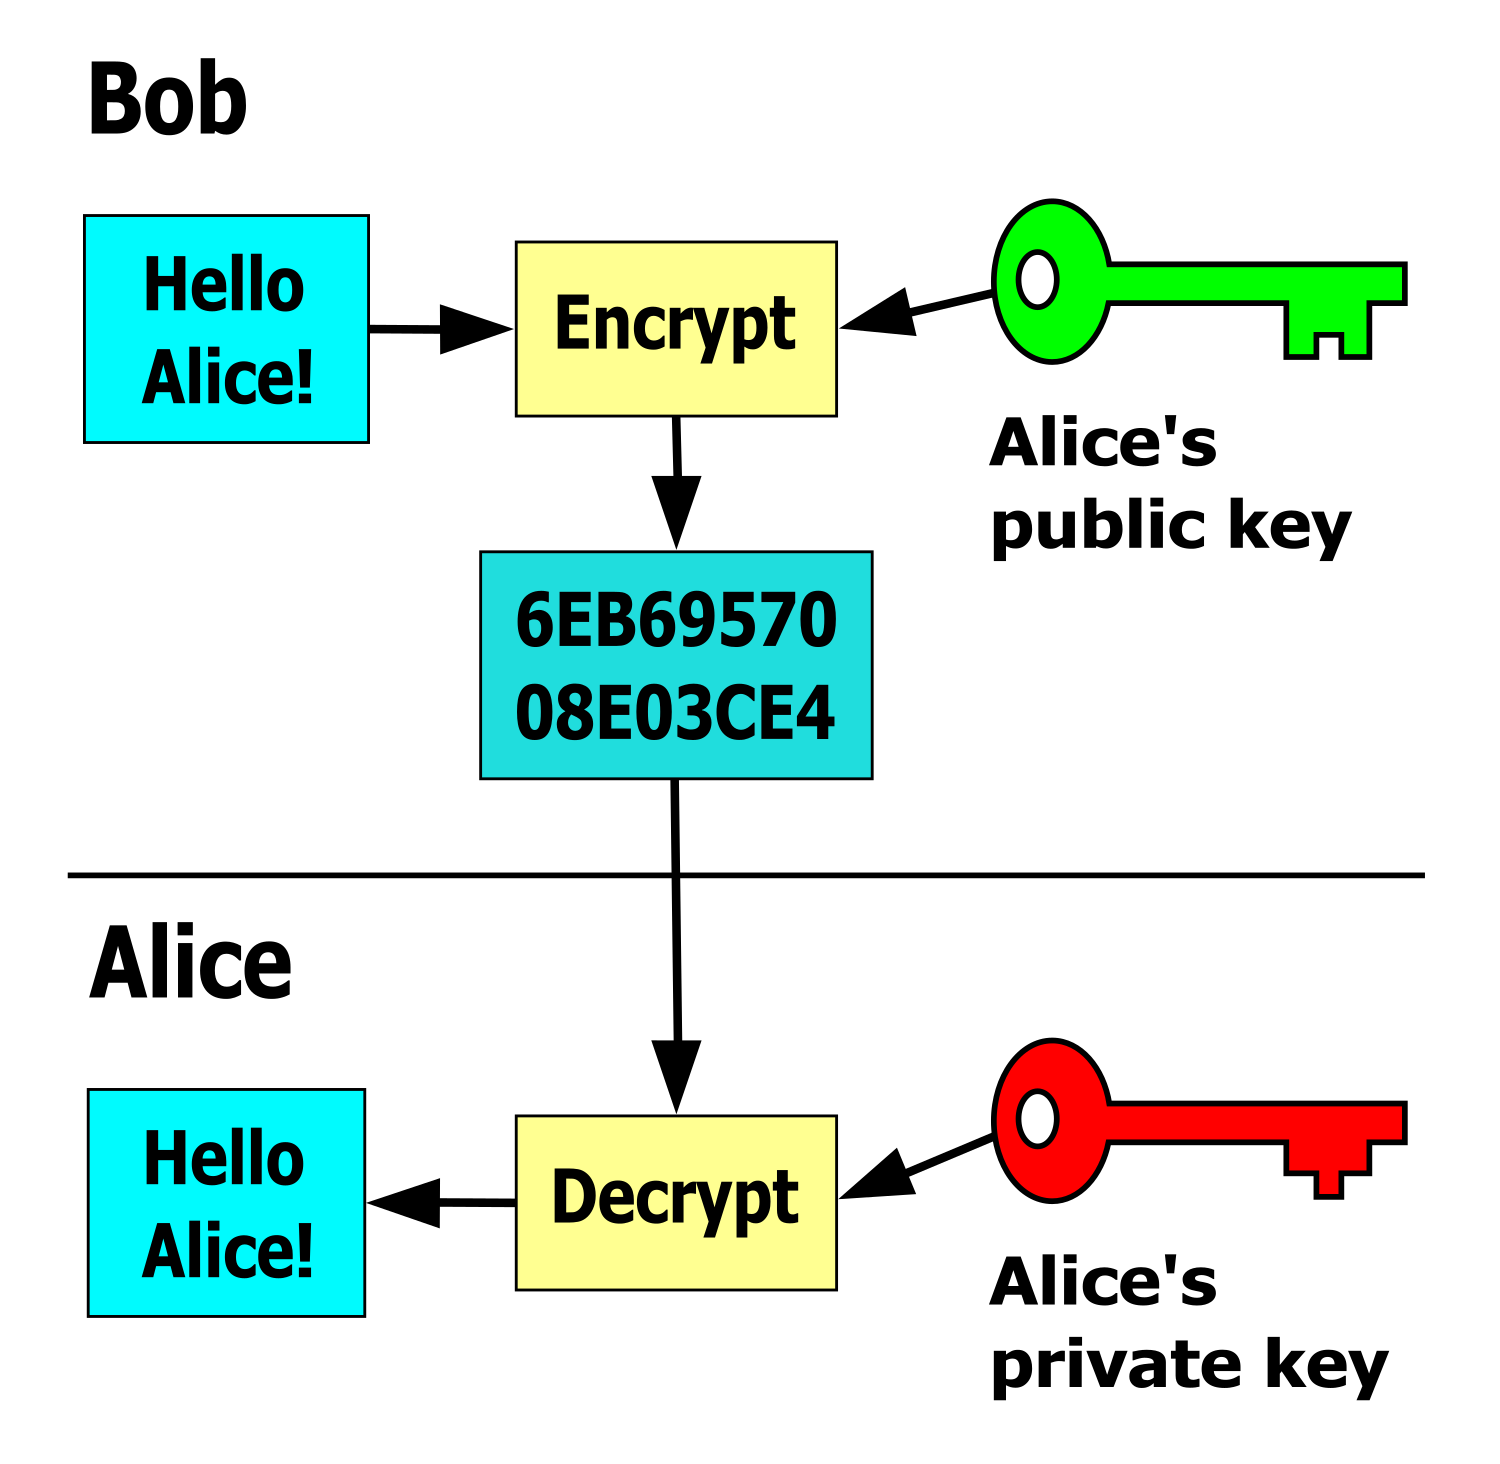
\includegraphics[width=0.5\textwidth]{images/public-key-encryption.png}
    \caption{Verschlüsselung mit Schlüsselpaaren}
\end{figure}

\clearpage

\subsection{Digitale Signaturen}

\subsubsection{Das Authentizitätsproblem}

Wenn Alice und Bob ihre Schlüssel ausgetauscht haben, kann niemand ihre Nachrichten mitlesen.
Doch fängt jemand jeweils die öffentlichen Schlüssel von Bob und Alice bei der Übertragung ab,
so kann diese Person Beiden Nachrichten schicken, von denen diese denken, sie wärem vom
jeweils anderen.

\subsubsection{Lösung mit digitalen Signaturen und Hash-Werten}

Damit Alice und Bob sicher sein können, dass niemand ihre Nachrichten verändert oder
ihnen Falschnachrichten sendet, können diese ihre Nachrichten mit ihren Schlüsseln signieren.
Anstatt ihre Nachricht nur mit Bobs öffentlichem Schlüssel zu verschlüsseln, wendet Alice vorher noch
ihren Privaten Schlüssel auf die Nachricht an. Jede Person mit Alice öffentlichem Schlüssel
kann so feststellen, dass die Nachricht von ihr kommt. Würde man diese Nachricht mit Alice
öffentlichem Schlüssel entschlüsseln wollen, und es wäre ein anderer privater Schlüssel
verwendet worden (z. B. von Eve), so würde sich keine Nachricht ergeben und man wüsste,
dass diese Nachricht nicht von Alice sein kann. Anschließend verschlüsselt sie wie vorher
auch die Nachricht mit Bob öffentlichem Schlüssel, da diese sonst jeder mitlesen könnte.
Nur Bob kann nun die Nachricht entschlüsseln und anschließend kann er mit Alice öffentlichem
Schlüssel die Authentizität überprüfen. Nun kann niemand anderes Bob Nachrichten in Alice Namen
senden. Gleiches gilt nun natürlich auch für Alice.

\begin{lstlisting}[basicstyle=\small]
PubKeyBob (PrivKeyAlice (Alice Nachricht)) = Alice Nachricht verschlüsselt und signiert
PrivKeyBob (Alice Nachricht verschlüsselt und signiert) = Alice Nachricht signiert
PubKeyAlice (Alice Nachricht signiert) = Nachricht
\end{lstlisting}

Ist Alice Nachricht sehr groß und sie will nicht auf die komplette Nachricht
ihren privaten Schlüssel anwenden (z. B. aus Effizienzgründen), so kann sie
einen Hash-Wert (diese ist deutlich kürzer als die Nachricht) der Nachricht erstellen
und nur diesen signieren. Anschließend verschlüsselt sie dann die Nachricht und
den signierten Hash-Wert und schickt diese an Bob.
Bob weiß, dass nur Alice ihm diesen Hash-Wert übermittelt haben kann, und kann so
prüfen, ob der Hash-Wert zur Nachricht passt, also ob die Nachricht wirklich von Alice
ist. Dazu nutzt er die gleiche Hash-Funktion wie Alice und prüft, ob sein und der signierte
Hash-Wert der gleiche sind.

\subsubsection{Erklärung von Hash-Funktionen und Hash-Werten}

Eine Hash-Funktion erstellt zu einer Eingabe an Daten einen Hash-Wert fester Länge.
Für die gleichen Daten ist dieser Hash-Wert beim mehrmaligen ausführen der 
Funktion auf diese Daten immer gleich.
Bei einer guten, kryptographisch sicheren Hash-Funktionen haben nahezu nie verschiedene
Daten den gleichen Hash-Wert und eine Umkehr der Funktion ist nicht einfach möglich.
Dadurch wird verhindert, dass man zu einem Hash-Wert einfach die Daten finden kann, die
diesen erzeugen.

\subsection{Zertifikate}

\subsubsection{Das Integritätsproblem}

Jetzt schaltet sich jedoch Eve dazwischen und startet einen Man-in-the-Middle Angriff.
Sie fängt die öffentlichen Schlüssel von Bob und Alice bei der Übertragung
ab und ersetzt diese durch einen öffentlichen Schlüssel eines anderen Schlüsselpaars (links).
Da Eve dazwischen geschaltet ist, kann sie jede Nachricht nun abfangen, entschlüsseln, lesen
und verändern (rechts). Anschließend sendet sie die Nachricht mit dem abgefangenen, echten öffentlichen
Schlüssel weiter an Bob bzw. Alice. Auch eine digitale Signatur von Alice auf die ganze Nachricht bringt nichts,
da Eve diese entschlüsseln kann und dann mit ihrem privaten Schlüssel eine neue
Signatur für Bob erstellt.

\vspace*{0.5cm}

\begin{center}
\adjustbox{scale=1.0}{
\begin{tikzpicture}
% left %
% alice
\draw (0,0) rectangle (4,2);
\node[draw] at (2,1.5) {Alice};
\node[draw=red, thick, rounded corners, fill=red!20] at (1,0.7) {Pub};
\node[draw=red, thick, rounded corners, fill=red!20] at (3,0.7) {Priv};
% eve
\draw (0,4) rectangle (4,6);
\node[draw] at (2,5.5) {Eve};
\node[draw=violet, thick, rounded corners, fill=violet!20] at (1,4.7) {Pub};
\node[draw=violet, thick, rounded corners, fill=violet!20] at (3,4.7) {Priv};
% bob
\draw (0,8) rectangle (4,10);
\node[draw] at (2,9.5) {Bob};
\node[draw=green, thick, rounded corners, fill=green!20] at (1,8.7) {Pub};
\node[draw=green, thick, rounded corners, fill=green!20] at (3,8.7) {Priv};
% arrows
\draw [-{Latex[length=2mm]}] (1,4) -- (1,2);
\draw [-{Latex[length=2mm]}] (3,2) -- (3,4);
\draw [-{Latex[length=2mm]}] (1,8) -- (1,6);
\draw [-{Latex[length=2mm]}] (3,6) -- (3,8);
% labels
\node[draw=red, thick, rounded corners, fill=red!20] at (3,3) {Pub};
\node[draw=violet, thick, rounded corners, fill=violet!20] at (1,3) {Pub};
\node[draw=violet, thick, rounded corners, fill=violet!20] at (3,7) {Pub};
\node[draw=green, thick, rounded corners, fill=green!20] at (1,7) {Pub};

% right %
% alice
\draw (6,0) rectangle (10,2);
\node[draw] at (8,1.5) {Alice};
\node[draw=red, thick, rounded corners, fill=red!20] at (7,0.7) {Priv};
\node[draw=violet, thick, rounded corners, fill=violet!20] at (9,0.7) {Pub};
% eve
\draw (6,4) rectangle (10,6);
\node[draw] at (8,5.5) {Eve};
\node[draw=red, thick, rounded corners, fill=red!20] at (6.8,4.6) {Pub};
\node[draw=violet, thick, rounded corners, fill=violet!20] at (6.8,5.4) {Priv};
\node[draw=violet, thick, rounded corners, fill=violet!20] at (9.2,4.6) {Priv};
\node[draw=green, thick, rounded corners, fill=green!20] at (9.2,5.4) {Pub};
% bob
\draw (6,8) rectangle (10,10);
\node[draw] at (8,9.5) {Bob};
\node[draw=violet, thick, rounded corners, fill=violet!20] at (7,8.7) {Pub};
\node[draw=green, thick, rounded corners, fill=green!20] at (9,8.7) {Priv};
% arrows
\draw [red, -{Latex[length=2mm]}] (7,4) -- (7,2);
\draw [violet, -{Latex[length=2mm]}] (9,2) -- (9,4);
\draw [violet, -{Latex[length=2mm]}] (7,8) -- (7,6);
\draw [green, -{Latex[length=2mm]}] (9,6) -- (9,8);

\end{tikzpicture}
}
\end{center}

\clearpage

\subsubsection{Lösung mit Zertifikaten und Zertifikatsstellen}

Bob hat eine Bank gegründet, bei der Alice Kundin ist. Damit Eve ihre vertrauliche Kommunikation
nicht mithören kann, nutzt Bob ein Zertifikat für seine Bank.
Nachdem Bob sein Schlüsselpaar generiert hat, hat er bei der Zertifikatsstelle ein Zertifikat
beantragt. Dazu musste er sich bei der Zertifikatsstelle authentifizieren, dass er
wirklich der Betreiber von Bob's Bank ist. Anschließend hat die Zertifikatsstelle ein
Zertifikat für seine Bank erstellt, in welchem sein öffentlicher Schlüssel sowie Informationen
über seine Bank mit dem privaten Schlüssel der Zertifizierungsstelle signiert ist.
Dieses sendet Bob nun an Alice, um zu bestätigen, dass sie wirklich mit Bob's bank kommuniziert.
Alice kann die Signatur des Zertifikats prüfen, da sie im voraus den öffentlichen Schlüssel
von der Zertifikatsstelle erhalten hat. Sie weiß dann, ob sie wirklich Bob's öffentlichen
Schlüssel erhalten hat. Eve kann kein Zertifikat für Bob's Bank beantragen, da sie sich
dafür bei der Zertifizierungsstelle als Bob authentifizieren müsste.
Beantragt sie ein anderes Zertifikat, so erkennt Alice, dass dieses nicht für Bob's Bank,
sondern für jemand anderen ausgestellt ist.
Erstellt Eve selbst ein Zertifikat, so erkennt Alice mit dem öffentlichen Schlüssel der
Zertifizierungsstelle, dass dieses gefälscht ist.
Dies funktioniert allerdings nur, weil Bob und Alice beide Faythe, dem Betreiber
der Zertifikatsstelle vertrauen und weil dieser sehr gewissenhaft arbeitet.
Da Alice Kunding bei Bob ist, kann sie sich über die gesichterte Verbindung nun mit ihrem
Password authentifizieren. Da sie den öffentlichen Schlüssel aus dem Zertifikat nutzt weiß sie,
dass nur Bob die Nachricht lesen kann.
Unter anderen Umständen, z. B. bei der Kommunikation zwischen Servern in einem Unternehmen
ist es auch möglich, dass diese sich gegenseitig Zertifikate zusenden.

\clearpage

\vspace*{2.5cm}

\begin{center}
\adjustbox{scale=1.4}{
\begin{tikzpicture}
% left %
\draw (-1,6) rectangle (4,8);
\node[draw] at (1,7.5) {Zertifikatsstelle};
\node[draw=yellow, thick, rounded corners, fill=yellow!20] at (0,6.7) {Pub};
\node[draw=yellow, thick, rounded corners, fill=yellow!20] at (3.3,6.7) {Priv};
% right %
% alice
\draw (6,0) rectangle (10,2);
\node[draw] at (8,1.5) {Alice};
\node[draw=red, thick, rounded corners, fill=red!20] at (7,0.7) {Priv};
\node[draw=red, thick, rounded corners, fill=red!20] at (9,0.7) {Pub};
\draw (6,-2.1) rectangle (10, -0.1);
\node[draw] at (8,-0.6) {Prüfschlüssel};
\node[draw=yellow, thick, rounded corners, fill=yellow!20] at (7,-1.4) {Pub};
% bob
\draw (6,7) rectangle (10,10);
\node[draw] at (8,9.5) {Bob's Bank};
\node[draw=green, thick, rounded corners, fill=green!20] at (7,8.7) {Pub};
\node[draw=blue, thick, rounded corners, fill=blue!20] at (7,7.7) {Cert};
\node[draw=green, thick, rounded corners, fill=green!20] at (9,8.7) {Priv};
% arrows
\draw [-{Latex[length=2mm]}] (9,2) -- (9,7);
\draw [-{Latex[length=2mm]}] (7,7) -- (7,2);
\node at (4.3, 9) {beantragt};
\draw [-{Latex[length=2mm]}] (6.45,8.7) -- (3.3, 8.7) -- (3.3, 7);
\node at (4.3, 3.7) {stellt aus};
\draw [-{Latex[length=2mm]}] (3.3, 6.4) -- (3.3, 4) -- (5.5, 4) -- (5.5, 7.7) -- (6.45, 7.7);
\node at (0.8, -1.7) {verteilt};
\draw [-{Latex[length=2mm]}] (0, 6.4) -- (0, -1.4) -- (6.45, -1.4);
% labels
\node[draw=blue, thick, rounded corners, fill=blue!20] at (7,4.5) {Cert};

\end{tikzpicture}
}
\end{center}
